\documentclass{article}
\usepackage{fullpage}
\usepackage{lastpage}
\usepackage{fancyhdr}
\usepackage{amssymb}
\usepackage{amsmath}
\usepackage{graphicx,subcaption} 
\usepackage{mathtools}
\usepackage{enumerate}
\usepackage{xspace}
\usepackage{txfonts}
\begin{document}
\begin{center}
{\Large \textbf{CMPUT 656 Course Project: Learning What to Remember}}\\
{Kenny Young}
\end{center}
\section*{Introduction}
Most reinforcement learning techniques assume the environment has the Markov property, meaning that the future state is independent of the past states given the present state. Put another way this assumes the agent has all the information it needs to make an optimal decision at each time and therefore has no need to remember the past. This is however not realistic in general, realistic problems often require significant information from the past in order to make an informed decision in the present and there is often no obvious way to incorporate the relevant information into an expanded present state. It is therefore desirable to establish general techniques for learning a compact representation of the relevant details of the past (i.e. a memory, or learned state) in order to facilitate decision making in the present.
Most modern attempts to tackle this problem make use of variations of recurrent neural networks trained with back-propagation through time. This can work well for many tasks, but generally requires backpropagating many steps into the past which is not practical in an online reinforcement learning setting. In this work we attempt to address the problem of memory without explicit backpropagation through time. To do this we propose a method for learning over time which information should be written to and read from a lossy external memory and which information we can afford to ignore. If an RNN can be considered a working memory the technique presented here is more similar to episodic memory, choosing which complete states to remember and recall in order to perform the present task.

\section*{Problem}
As a proof of concept for our proposed method we propose a toy problem we call ``the secret informant problem'' which requires an agent to figure out what information from past states is informative about the correct decision to make in the future. The environment consists of a chain of states each represented by a feature vector. In each state k possible actions are available (we use k=3 throughout), however the action choice only changes the outcome in the final state where 1 of the three actions will yield a reward of $+1$ and the other 2 will yield $0$ reward. Which action will yield the reward is drawn uniformly for each episode of the problem and can be determined for a given episode only by looking at the feature vector of some past state (which we refer to as the informant state) prior to the state in which the choice must be made. The feature vector associated with each state is shown in figure \ref{fig:state}.

The agent starts with no knowledge of the semantic interpretation of the state representation and must learn through successive trials what information is relevant to allow it to select the correct action in the final state. It also does not initially know that reward is only available in the final state and all other actions are irrelevant so this too must be learned. An instance of the full problem is shown in \ref{fig:problem}.
\begin{figure}[!ht]
\center
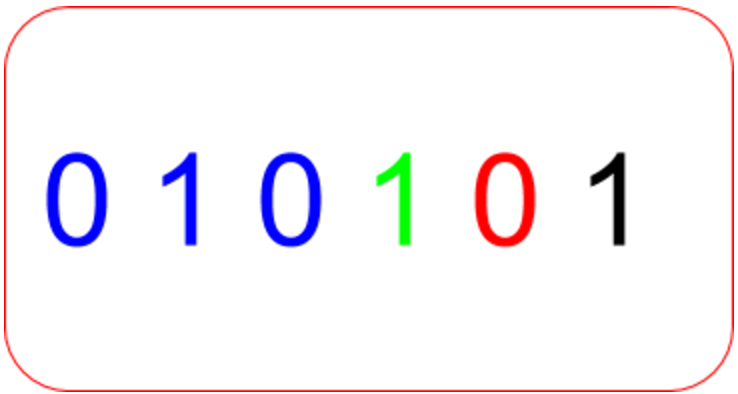
\includegraphics[width=0.5\textwidth]{images/state.png}
\caption{State representation for our test problem, blue digits are a one hot representation of which action the state is suggesting is correct (i.e. will yield $+1$ reward), the green digit will be 1 if and only if this state actually determines the correct action to take (i.e. it is the informant state). The red digit will be 1 if and only if the blue indicator is random and uncorrelated with the correct action choice (i.e. it is a noisy state). The final digit is simply an always on bias which may aid in the memory mechanism we will describe later. In addition to the general interpretation of these digits there is a special start node with code 000001 and the final node (at which the action choice will give a reward) with code 000011.}
\label{fig:state}
\end{figure}

\begin{figure}[!ht]
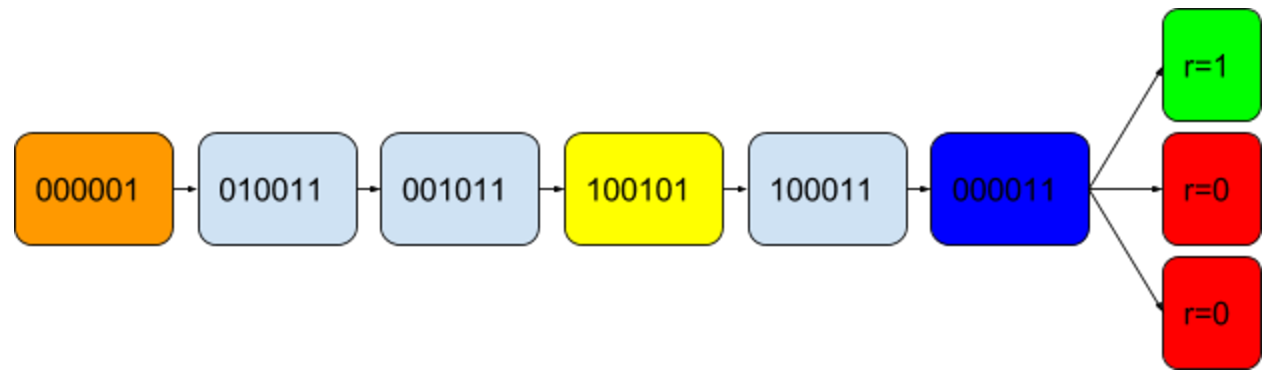
\includegraphics[width=1\textwidth]{images/problem.png}
\caption{An instance of the secret informant problem, the start state is orange, the final state (at which a decision must be made) is dark blue, the informant state (with the 4th bit set to 1) is yellow while the noisy states (with the 4th bit set to 0) are pale blue. Notice that because the 1st bit in the informant state is 1 and the rest are 0 the reward must be given for the top action and no other. In each instance of the problem the informant state will be placed randomly between the start and final state. Here we have 3 noisy states in addition to the informant state, in our tests we use 9 noisy states.}
\label{fig:problem}
\end{figure}

\section*{Related Work}

\section*{Proposed Method}
The main contribution of this work is to suggest a new kind of memory module designed to be trainable to both read and write using only information local in time (i.e. without requiring something like backpropagation through time). The instantiation of this idea presented here is meant only as a proof of concept with much room for improvement in terms of both theoretical foundation and actual implementation.
\subsection*{Memory Module}
The memory module is inspired by (though currently quite different from) the Holographic Reduced Representation used in \cite{LSTM}, and is intended to store and recall vectors of a fixed length $n$. It consists of $m$ complex copies, each of length $n$. Each time a write is performed it is accompanied by a positive weight $r$ (fixed here to be in $[0,1]$) which simply multiplies the item to be stored and corresponds to how strongly we wish to remember the current state. Additionally each copy is multiplied by a uniformly random complex phase $e^{i\theta_k}$ chosen separately for each copy stored. If we take the memory to be an $(m,n)$ complex matrix $M$ writing a vector $\pmb{s}$ with weight $r$ is done as follows:

$$M_{k,j}\mathrel{+}=re^{i\theta_k}\pmb{s}_j$$

Where here $j$ indexes the elements of the stored vector $\pmb{s}$ and $k$ indexes the $m$ copies stored in the memory. Now consider how we can go about recalling stored items from this memory. If we knew the set of random phases with which the desired item was stored $e^{i\theta_k}$ we can multiply each copy by its complex conjugate $e^{-i\theta_k}$ and take the real part of the result to retrieve an estimate $\pmb{u_{0k}}$ of $r\pmb{s}$. Since the phases used for all other stored items are uniformly random they will still be uniformly random when multiplied by $e^{-i\theta_k}$. i.e. for a particular $k$ and $\pmb{s_t}$ where $t$ is the time-step we wish to recover our written value from, and $\pmb{s_t}$ is the input state written to memory at that time we get an estimate that looks like this:
\begin{align*}
\pmb{u_{0k}}&=\Re(e^{-i\theta_{kt}}M_{k,:})\\
&=\Re(r_t\pmb{s_t}+\sum_{\tau\neq t}e^{i(\theta_{k\tau}-\theta_{kt})}r_\tau\pmb{s_\tau})\\
&=r_t\pmb{s_t}+\Re(\sum_{\tau\neq t}e^{i(\theta_{k\tau}-\theta_{kt})}r_\tau\pmb{s_\tau})\\
&=r_t\pmb{s_t}+(\textit{Expectation 0 Noise})
\end{align*}
By Averaging the resulting estimates $\pmb{u_{0k}}$ over all $m$ copies in memory we get a better unbias estimate $\pmb{u_0}$ of $r_t\pmb{s_t}$. In order to get rid of the scaling factor $r_t$ we enforce that all the $\pmb{s_t}$ are normalized before being written to memory, thus we simply normalize the resulting estimate of $r_t\pmb{s_t}$ to obtain an estimate $\pmb{u}$ of $\pmb{s_t}$ itself.

The bad news is we do not actually know the complex phases $e^{-i\theta_k}$ for the particular item we are trying to recall. The only information we are storing is the $m$ complex vectors that make up the memory. In the present work we use a particular method for querying the memory and estimating these phases, however the theoretical details have not been fully hashed out. Refining our memory mechanism to have better understood theoretical properties (which hopefully translates into better results and greater applicability) is a task for future work.

The way we handle queries to the memory is a form of content addressable read mechanism. A query to the memory consists of an arbitrary real vector of length $n$ (the same as the length of the stored items). For each copy in the memory we then estimate the phase of the desired read value to be the phase which results in the maximum dot product between the query $\pmb{q}$ and the returned estimate $\tilde{\pmb{s_t}}_{k}$. As we will now show this maximization process is a differentiable operation and can thus be trained by backpropagation directly.
\begin{align*}
\theta_k&=\underset{\theta}{argmax}\  \Re(e^{i\theta}\pmb{q}\cdot M_{k,:})\\
&=\underset{\theta}{argmax}\  \Re(\cos(\theta)\pmb{q}\cdot M_{k,:}+i\sin(\theta)\pmb{q}\cdot M_{k,:}\\
&=\underset{\theta}{argmax}\  \cos(\theta)\Re(\pmb{q}\cdot M_{k,:})-\sin(\theta)\Im(\pmb{q}\cdot M_{k,:})\\
&\implies \frac{d}{d\theta}\left(\cos(\theta)\Re(\pmb{q}\cdot M_{k,:})-\sin(\theta)\Im(\pmb{q}\cdot M_{k,:})\right)=0\text{, at }\theta_k\\
&\implies -\sin(\theta_k)\Re(\pmb{q}\cdot M_{k,:})-\cos(\theta_k)\Im(\pmb{q}\cdot M_{k,:})=0\\
&\implies \tan(\theta_k)=-\frac{\Im(\pmb{q}\cdot M_{k,:})}{\Re(\pmb{q}\cdot M_{k,:})}\\
&\implies \theta_k=n\pi-\arctan\left(\frac{\Im(\pmb{q}\cdot M_{k,:})}{\Re(\pmb{q}\cdot M_{k,:})}\right)\text{, for some integer }n
\end{align*}
Note that angles differing by $2\pi$ are equivalent hence there are really 2 extrema here, one is a minimum and one is a maxima. To figure out which is which we can look at the second derivative. After doing this and performing some simple algebra we find that the maxima we desire is given by:
$$\theta_k = \begin{cases}
 -\arctan\left(\frac{\Im(\pmb{q}\cdot M_{k,:})}{\Re(\pmb{q}\cdot M_{k,:})}\right) &\text{if $\Re(\pmb{q}\cdot M_{k,:})\geq0$}\\    \pi-\arctan\left(\frac{\Im(\pmb{q}\cdot M_{k,:})}{\Re(\pmb{q}\cdot M_{k,:})}\right) &\text{if $\Re(\pmb{q}\cdot M_{k,:})<0$}
\end{cases}
$$
We can use this angle to find the estimated $\pmb{s}$ in memory ``closest'' to the query $\pmb{q}$ as described above. Note that since this optimal angle and the subsequent computation of the estimate $\pmb{s}$ described above are both differentiable almost everywhere, we can backpropogate through this to improve our generated queries $\pmb{q}$ in order to make use of our stored memories to achieve our specified task. We refer to the estimated $\pmb{s}$ recovered by this process (i.e. the value retrieved from memory in response to query $\pmb{q}$) as $\pmb{u}$.

\subsection*{Training Write Network}
As highlighted above the query portion of our network is fully differentiable and therefore trainable directly by backpropagation. In addition we have a second network whose purpose is to choose the write weight $r$ for the state at each time-step. While in principle the write portion of the network is also differentiable and could also be trained by a variant of backpropagation through time, the purpose of the present work is to design a method which avoids this, thus we instead use an update method which is strictly local in time. Our method attempts to approximate $\frac{d\sigma^2(Q(\pmb{s},a))}{dr(\pmb{u})}$ (i.e. the change in the variance of each action value in the current state over the change in the write weight associated with the current read value). Using this estimate we then compute $\frac{d\sigma^2(Q(\pmb{s},a))}{\theta_{write}}=\frac{d\sigma^2(Q(\pmb{s},a))}{dr(\pmb{u})}\frac{dr(\pmb{u})}{\theta_{write}}$ for each parameter $\theta_{write}$ of the write network. This value is then used to perform gradient descent to tune the write network to generate weights which produce low average variance in the computed action values over all actions.

To approximate $\frac{d\sigma^2(Q(\pmb{s},a))}{dr(\pmb{u})}$ we first assume $\sigma^2(Q(\pmb{s},a)) = \left(\frac{dQ(\pmb{s},a)}{d\pmb{u}}\right)^2\sigma^2(\pmb{u})$, which is an assumption commonly employed to perform propagation of experimental errors in the physical sciences. Differentiating with respect to $r$ then gives us: 
$$\frac{d\sigma^2(Q(\pmb{s},a))}{dr} = \left(\frac{dQ(\pmb{s},a)}{d\pmb{u}}\right)^2\frac{d\sigma^2(\pmb{u})}{dr(\pmb{u})}$$
$\frac{dQ(\pmb{s},a)}{d\pmb{u}}$ is easily computed by ordinary backpropagation, but it remains to estimate $\frac{d\sigma^2(\pmb{u})}{dr(\pmb{u})}$. Since $\pmb{u}$ is generated from $m$ independent estimates, we can approximate $\sigma^2(\pmb{u})$ as the standard error in the mean computed from these $m$ samples. Approximating its derivative with respect to $r(\pmb{u})$ requires a bit more creativity. To do this we take $\pmb{u}$ to be the ``true'' value and take the difference of the estimates directed from individual samples from this value to be added noise terms $\pmb{\mathcal{N}_k}$ defined as follows:
\begin{align*}
\pmb{u_0}&=\frac{1}{m}\sum_{k=1}^m\pmb{u_{0k}}\\
\bar{r}&=|\pmb{u_0}|_2\\
\pmb{u}&=\frac{\pmb{u_0}}{\bar{r}}\\
\pmb{u_k} &= \frac{\pmb{u_{0k}}}{\bar{r}}\\
\pmb{\mathcal{N}_k}&=\pmb{u_{0k}}-\pmb{u_0}\\
\implies\pmb{u_{0k}}&=\pmb{u_0}+\pmb{\mathcal{N}_k}
\end{align*}
We then make the assumption that $\pmb{u}$ does in fact correspond to an actual value $\pmb{s}$ which was written to the memory, plus some additive noise with some $r=\bar{r}$ which can be estimated as the magnitude of $\pmb{u_0}$ ($\pmb{u}$ prior to normalizing). Given this we can reasonably assume that the modifying $r(\pmb{u})$ to a value other than $\bar{r}$ will change the magnitude of $\pmb{u_o}$ while holding the added noise terms $\pmb{\mathcal{N}_k}$ constant. Hence letting $\pmb{u_o}(r)$ be the scaled value of $\pmb{u_o}$ at a new $r$ value, we arrive at the following expression for $\pmb{u_k}(r)$ (the $k_{th}$ sampled estimate of $\pmb{u}$).
\begin{align*}
\pmb{u_0}(r) &= \frac{\pmb{u_0}r}{\bar{r}}\\
\pmb{u_{ok}}(r) &= \pmb{u_0}(r)+\pmb{\mathcal{N}_k}\\
&=\frac{\pmb{u_0}r}{\bar{r}}+\pmb{\mathcal{N}_k}\\
\pmb{u_k}(r) &= \frac{\pmb{u_{ok}}(r)}{r}\\
&= \frac{\pmb{u_0}}{\bar{r}}+\frac{\pmb{\mathcal{N}_k}}{r}\\
&=\pmb{u}+\frac{\pmb{\mathcal{N}_k}}{r}
\end{align*}
So the final result is just that the difference in each sampled estimate from the mean is divided by $r$ instead of $\bar{r}$. From this we can compute an estimate of $\sigma^2(\pmb{u}(r))$ as a function of r as follows:
\begin{align*}
\sigma^2(\pmb{u}(r))&=\frac{1}{m}\sum_{k=1}^m(\pmb{u}-\pmb{u}_k(r))^2\\
&=\frac{1}{m}\sum_{k=1}^m\left(\frac{\pmb{\mathcal{N}_k}}{r}\right)^2
\end{align*}
And finally we can differentiate this approximation with respect to $r$ to yield:
$$\left.\frac{d\sigma^2(\pmb{u})}{dr}\right\rvert_{\bar{r}}=-\frac{2}{m}\sum_{k=1}^m\frac{\pmb{\mathcal{N}_k}^2}{\bar{r}^3}$$
At this point we now have all the ingredients to estimate $\frac{d\sigma^2(Q(\pmb{s},a))}{\theta_{write}}$ for a particular read value $\pmb{u}$ at a particular time-step. Not however that there is a hidden tradeoff, because the nature of the memory is that each written item interfere with all others. Hence if we increase the write weight assigned to one particular input state $\pmb{s}$ it will also increase the noise terms associated with all other written values. Applying the above approximate gradients naively will lead to all write weights gradually increasing (though at differing rates), which is not acceptable. To counter this, for now, we simply maintain an exponential moving average of $\frac{d\sigma^2(Q(\pmb{s},a))}{dr}$ and subtract this from the value at each time-step before performing the gradient descent update. This means that the write weight associated with the current read value $\pmb{u}$ will be increased only if it's associated $\frac{d\sigma^2(Q(\pmb{s},a))}{dr(\pmb{u})}$ surpasses the current moving average and will be decreased otherwise. To summarize we use:
\begin{align*}
\text{Effective Gradient}&=\left(\left(\frac{dQ(\pmb{s_t},a)}{d\pmb{u_t}}\right)^2\frac{d\sigma^2(\pmb{u_t})}{dr(\pmb{u_t})}-S_t\right)\frac{dr(\pmb{u_t})}{\theta_{write}}\\
S_{t+1} &=\alpha\left(\left(\frac{dQ(\pmb{s_t},a)}{d\pmb{u_t}}\right)^2\frac{d\sigma^2(\pmb{u_t})}{dr(\pmb{u_t})}\right)+(1-\alpha)S_t
\end{align*}
Where each term is approximated as discussed above, and we insert this ``effective gradient'' as the gradient for some gradient descent optimizer acting on all $\theta_{write}$ parameters of the write network at each time-step. In our experiments we use $\alpha=0.5$ in the moving average.

\subsection*{Architecture}
Our architecture for interacting with the memory and generating action values is shown in Figure \ref{fig:arch}. It consists of 4 major parts. Except where otherwise specified all activations are rectified linear.

First is the query network which takes the state itself as input and consists of 2 relu layers followed by an identity layer which generates the query which is sent to the memory. Additionally the $2_{nd}$ layer of the query network is passed forward so that information about the current state is available for computing action values. 

Second we have the memory itself which works as described above receiving queries $\pmb{q}$ from the query network and writes $\pmb{v_k}=re^{i\theta_k}\pmb{s}$, and sending responses $\pmb{u}$ to the action value network.

Third is the action value network itself which takes the memory responses along with information about the current state from the $2_{nd}$ layer of the query network and generates estimated values for each of the 3 actions. The action values in this case are bounded between 0 and 1 (in fact the true action values are either 0 or 1), hence the output of the action value network uses a sigmoid activation. The action value network is trained using deep Q-learning and propagates gradients directly through the memory to improve the $\pmb{q}$ values produced, as well as along the path directly to the input without passing through the memory.

Last we have the write network which is trained entirely separately from the others and outputs a single sigmoid activation $r$. This $r$ is multiplied by the normalized input along with a separately drawn uniformly random complex phase for each copy stored in the memory. The training process for the write network is described in detail in the memory section above.

\begin{figure}[!ht]
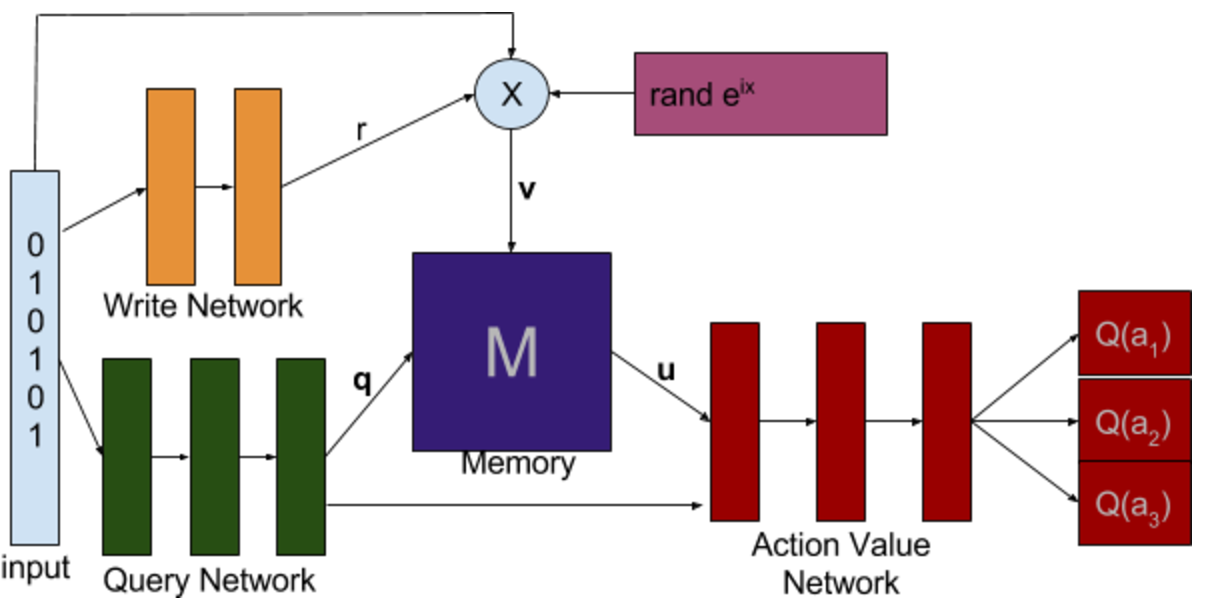
\includegraphics[width=1\textwidth]{images/architecture.png}
\caption{Our architecture, input is given separately to both query and write network. Write network output is sigmoid to give a weight between 0 and 1, this weight multiplies the input vector input along with a random complex phase to give the value that is actually written to memory. The query network output \textbf{q} to memory is identity (i.e. potentially spans the whole space) the memory returns a vector \textbf{u}. The input to the action value network consists of the output of the second last layer of the query network, along with the value \textbf{u} read from memory. The action value network outputs action values for all available actions.  }
\label{fig:arch}
\end{figure}

\section*{Results}
We run experiments on the secret informant problem (see Figure \ref{fig:problem}) with 4 noisy states and run for 50,000 episodes. Each layer of our model uses 15 units. We use Nesterov Momentum as our optimizer for both the write and action evaluation portions of the network as it was found to be reasonably stable compared to some other options tried. Learning rates were tuned by hand to achieve reasonable performance, it was found that in general training the write network with around $1/10_{th}$ the learning rate of the action evaluation network worked well. We use a memory with just 3 copies in our experiments. Results for 50 repetitions of this experiment, including the output of the write network in the informant state v.s. the average over all other states, are shown in Figure \ref{fig:1_query}.

In addition to this main model we test two baselines. First to test the efficacy of the write network we run the model with $r$ fixed to 1 and the write network disabled. This means each visited state is written to the memory with equal intensity. Second we run a model with essentially the same architecture as our action evaluation network but with the memory replaced by a GRU with 5 recurrent units trained using standard backpropagation through time. This last model is meant to give an idea of how difficult the task is for a traditional recurrent architecture but as it hasn't been all that thoroughly tuned it is not a very rigorous baseline. It should also be noted that our goal in this work was to avoid the need to perform backpropagation through time explicitly so any comparison there is not really fair. Figure \ref{recurrent} shows  

We also experimented with variants of our architecture which allowed for multiple queries on each time step which appeared in initial tests to speed up early learning somewhat, however it has so far been prone to instability so results are not included here. This would be more useful in cases where it is actually necessary to query the values of two distinct past states to make a decision in the current state.
\begin{figure}[!ht]
\centering
\begin{subfigure}[t]{.45\textwidth}
  \centering
      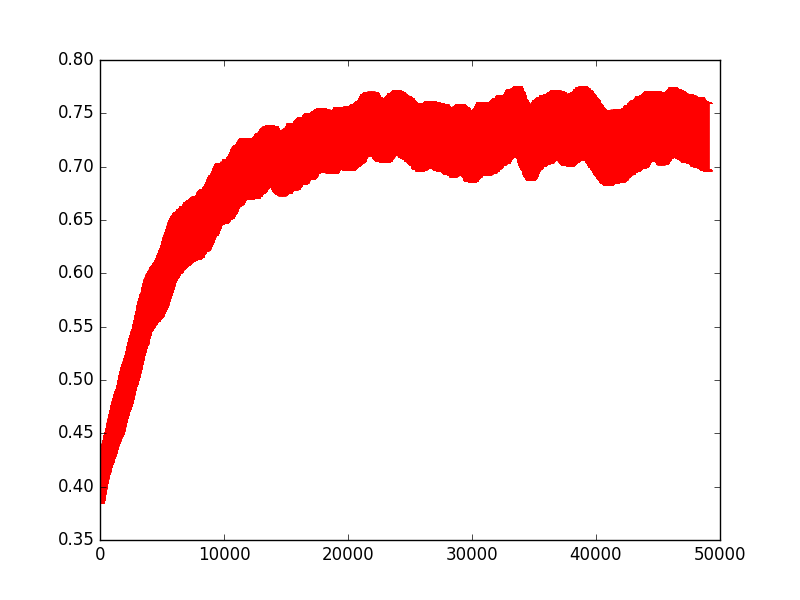
\includegraphics[width=1\textwidth]{images/1_query_mem_ret.png}
  \caption{Returns over time for memory based architecture. y-axis is return, x-axis is number of training episodes.}
  \label{fig:1_query_ret}
\end{subfigure}\hfill
\begin{subfigure}[t]{.45\textwidth}
  \centering
      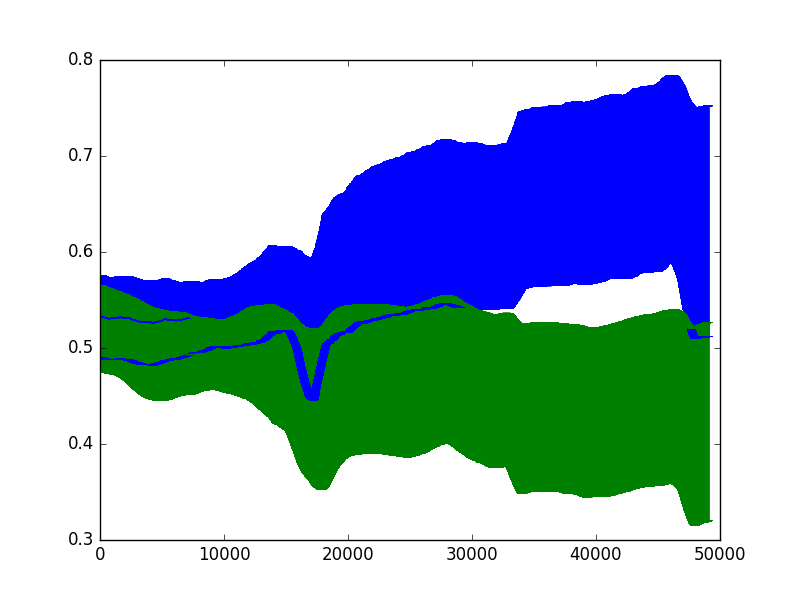
\includegraphics[width=1\textwidth]{images/1_query_mem_writes.png}
  \caption{Write weight for informant state (blue) and average write weight for all other states (green). y-axis is write weight, x-axis is number of training episodes.}
  \label{fig:1_query_write}
\end{subfigure}
\caption{Results for memory based architecture. In each case displayed results are averaged over 50 runs with the width of the curve indicating standard error in the mean.}
\label{fig:1_query}
\end{figure}

\begin{figure}[!ht]
\center
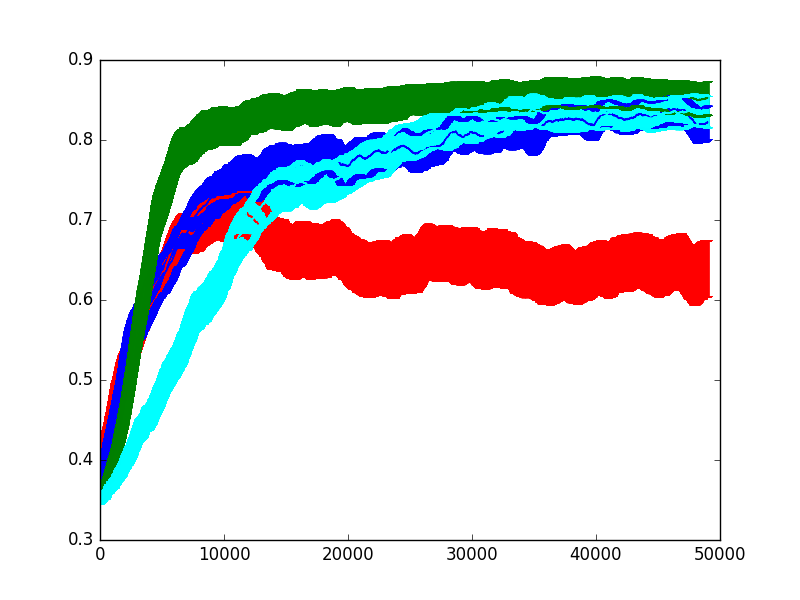
\includegraphics[width=0.5\textwidth]{images/combined_ret.png}
\caption{Returns over time for memory based architecture and two baselines. Main memory based architecture with write weight tuning is shown in red, memory based architecture with write weight tuning disabled is shown in blue, recurrent architecture is shown in green. y-axis is return, x-axis is number of training episodes.}
\label{fig:comparison}
\end{figure}

\section*{Discussion}
The results are mixed in terms of demonstrating the feasibility of our suggested memory system and write weight training. While Figure \ref{fig:1_query_write} suggests our write weight training mechanism is able to learn to separate informative from uninformative states, we can see in Figure \ref{fig:comparison} that our write weight tuning nevertheless hurts performance compared to simply fixing all write weights at 1. The reason for this is likely that although on average we learn to write useful states more strongly the variance over runs is extremely high and occasionally the useful states do end up being written significantly less strongly. What is likely happening is that the performance cost of these occasional failures is high enough compared to the gain from the more frequent successes that overall performance is hindered. 

Our system also seems to lose out somewhat to a standard recurrent architecture, however this in itself is not too meaningful as our purpose here is to explore memory mechanisms which avoid the need to perform explicit backpropagation through time which is exactly what is done by the recurrent model tested.

It should be noted that the mechanism presented here for training the write network is not particular to the memory system used here but is actually quite broadly applicable. Essentially all that is required to use our write weight training algorithm is a system with roughly the following components:
\begin{itemize}
\item A memory is capable of storing and recalling vectors with a tuneable fidelity parameter, where improved recall of one memory will hurt can be traded off for poor recall of others
\item A differentiable function mapping the recalled memory to some value whose variance we wish to minimize (in our case learned action values)
\item A way of estimating the derivative of standard error in the mean of a value read from memory with respect to it's associated fidelity parameter at write time(in our case we use an approximated derivative of the sample standard deviation over several independent copies)
\end{itemize}
Thus despite the failure of the tuned write weights to aid in performance we are encouraged by the evidence of our ability to successfully tune write weights based on utility of the information contained in a state.

\section*{Conclusion}

\section*{Limitations and Future Work}
This work is intended primarily as a proof of concept for systems the operate on some form of variable fidelity memory mechanism and learn write weights based on how the read values impact a systems ability to consistently achieve some primary task. As such there are likely numerous theoretical and practical improvements that could be made, as well as far more empirical testing that to be done. 

First of all the memory mechanism itself is far from perfect. Significant improvement could likely be derived from more thorough theoretical investigation of such mechanisms and more precise formulation of exactly what properties we would like the memory to display. Under the current mechanism it is not clear at all how we should interpret the read value when the query made has a nonzero dot-product with multiple previously written values which is something we hope to improve on through more investigation.




\begin{thebibliography}{plain}
\bibitem{NTM}
Graves, A., Wayne, G., and Danihelka, I. (2014) Neural Turing Machines. arXiv preprint arXiv:1410.5401.

\bibitem{MC}
Oh, J., Chockalingam, V., Singh, S., and Lee, H. (2016) Control of Memory, Active Perception, and Action in Minecraft. ICML, New York City, 2016. JMLR Workshop and Conference Proceedings Volume 48.

\bibitem{LSTM}
Danihelka, I., Wayne, G., Uria, B., Kalchbrenner, N., and Graves, A. (2016) Associative Long Short-Term Memory. ICML, New York City, 2016. JMLR Workshop and Conference Proceedings Volume 48.

\bibitem{DNC}
Graves, A. et al. (2016) Hybrid Computing Using a Neural Network with Dynamic External Memory. Nature 538, 471-476.

\bibitem{RARE}
Kaiser, Lukasz, et al. (2017) Learning to remember rare events. arXiv preprint arXiv:1703.03129.
\end{thebibliography}



\end{document}